\section{Distributed Processing of Spatial Algorithms}
\label{sec:spatial_dist}

\subsection{Data Structures for Spatial Data Processing}
\label{sub:spatialdata}		
A number of structures have been proposed for handling multi-dimensional point data, such as: KD-Tree \cite{bentley1975multidimensional}, Hilbert R-Tree \cite{kamel1994hilbert} and R-Tree \cite{guttman1984r}.

An R-Tree is a height-balanced tree similar to a B-Tree \cite{comer1979ubiquitous} with index records in its leaf nodes containing pointers to data objects. 
The key idea of the data structure is to group nearby objects and represent them with their minimum bounding rectangle (MBR) in the next higher level of the tree. 

Figure \ref{fig:rtree} illustrates the hierarchical structure of an R-Tree with a root node, internal nodes ($N1...2 \subset N3...6$) and leaves ($N3...6 \subset a...h$). 
The Figure \ref{fig:rtree-space} shows MBRs grouping spatial objects of $a...h$ in sets by their co-location. 
The Figure \ref{fig:rtree-index} illustrates the R-Tree representation. Each node stores at most $M$ and at least $m \leq M/2$ entries [Guttman 1984].

\begin{figure}[h]
  \centering
  \subfigure[R-Tree index]
  {
  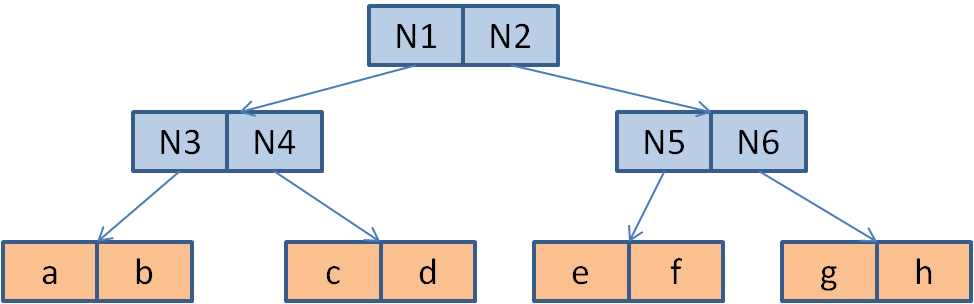
\includegraphics[width=0.45\textwidth]{rtree}
  \label{fig:rtree-index}
  } \qquad
  \subfigure[Geographic space]
  {
  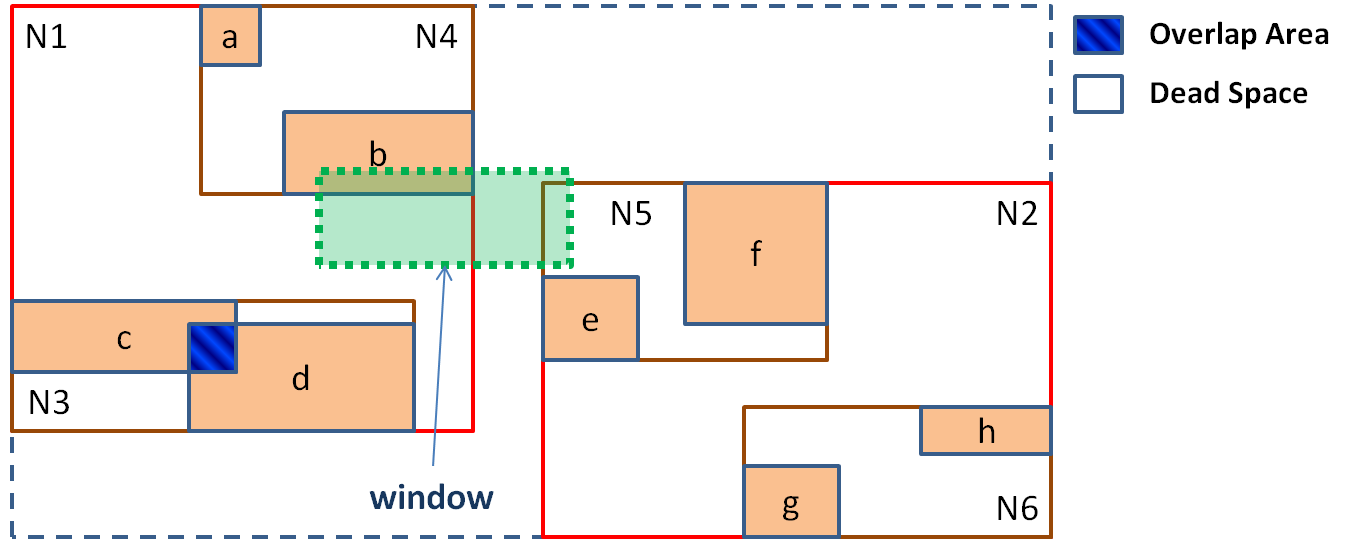
\includegraphics[width=0.45\textwidth]{rtree-space}
  \label{fig:rtree-space}
  }
  \caption{R-Tree Structure}
  \label{fig:rtree}
\end{figure}

The Window Query is one of major query algorithms in R-Tree. The input is a search rectangle (Query box). The search starts from the root node of the tree. 
Every internal node contains a set of rectangles and pointers to the corresponding child node and every leaf node contains the rectangles of spatial objects (the pointer to some spatial object can be there). 

For every rectangle in a node, it has to be decided if it overlaps the search rectangle or not. If yes, the corresponding child node has to be searched also. 
Searching is done recursively until all overlapping nodes have been traversed. When a leaf node is reached, the contained bounding boxes (rectangles) are tested against the search rectangle 
and their objects (if there are any) are put into the result set if they lie within the search rectangle.

In Figure \ref{fig:rtree}, the search starts on root node, where window intersects with the N1 and N2 nodes. Then, the algorithm analyze N4 and N5 entries in N1 node, in which only N4 intersects with the window. 
Analyzing N4, the algorithm returns the object namely 'b', that is the single object that intersects the window.

In N2, none entry intersects with the window. This happens because of dead space, in other words, the window intersects with a space which not contains any data. 
The dead space should be minimized to improve the query performance, since decisions which paths have to be traversed can be taken on higher levels. 

The overlap area between rectangles should be minimized too because it degrades the performance of R-Tree \cite{beckmann1990r}. 
Less overlapping reduces the amount of sub-trees accessed during r-tree traversal. The area between c and d in Figure \ref{fig:rtree} is an example of overlapping.

\subsection{DistGeo: A Platform of Distributed Spatial Operations for Geoprocessing}

This work developed a platform, namely DistGeo (Figure \ref{fig:dist}), to process the spatial operations in a cluster of computers. 
DistGeo is based on the shared-nothing architecture, which the nodes do not share CPU, hard disk and memory and the communication relies on message exchange. 
Figure \ref{fig: Figure 3} depicts DistGeo plataform based on peer-to-peer model, with the data manage by the cluster presented as a ring topology. 
It is divided in ranges of keys, which are managed for each node of the cluster. To a node join the ring it must first receive a range.

The range of keys are known by each node in the cluster. For instance, in a ring representation, whose key set start with 0 till 100, if we have 4 nodes in the cluster, the division could be done as shown below: 
a) 0-25, b) 25-50, c) 50-75 e d) 75-100. If we want to search for one object with key 34, we certainly should look on the node 2.

\begin{figure}[h]
  \centering
  \subfigure[DistGeo Architecture]
  {
  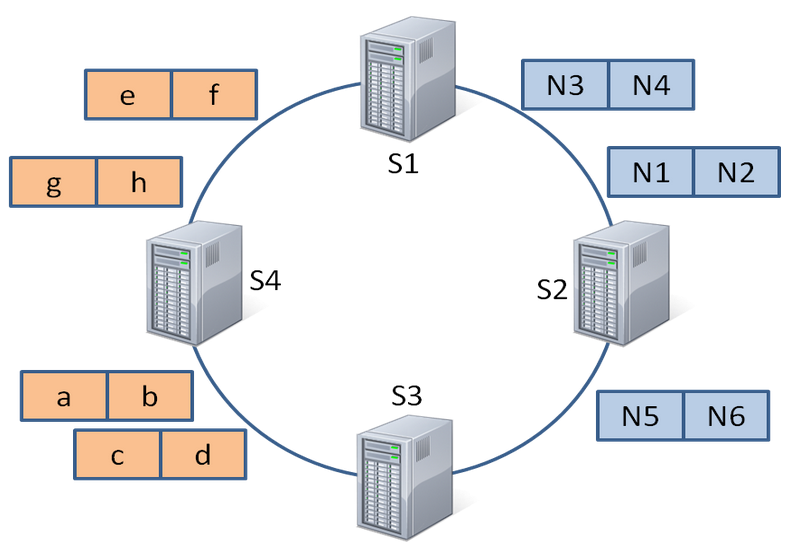
\includegraphics[width=0.45\textwidth]{figure3.png}
  \label{fig: Figure 3}
  } \qquad
  \subfigure[R-Tree Partitioning in DistGeo]
  {
  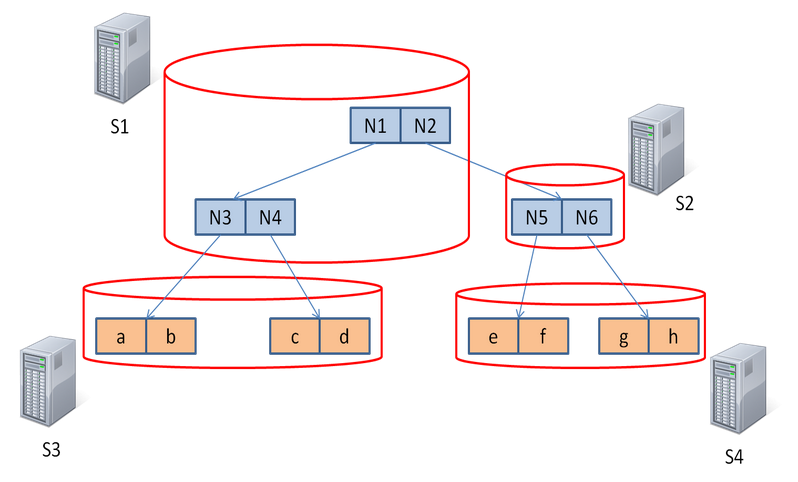
\includegraphics[width=0.45\textwidth]{r-tree-partiotioning.png}
  \label{fig:partitioning}
  }
  \caption{DistGeo Platform}
  \label{fig:dist}
\end{figure}
	
Every replica of an object is equally important, in other words, there is not a master replica. Read/Write operations may be performed in any node of the cluster. 
When a request is made to a cluster's node, it becomes the coordinator of the operation requested by the client. The coordinator works as a proxy between the client and the cluster's nodes. 
	
DistGeo utilizes the Gossip protocol, which every cluster node exchanges information among themselves for service discovery and knowing the statuses of the cluster's nodes. 
In the Gossip protocol every second a message is exchanged among three nodes in the cluster, consequently every cluster's node have knowledge of each other. 

Figure \ref{fig:partitioning} illustrates the structure of a Distributed R-Tree in a cluster. The partitioning it is performed grouping the nodes in cluster and creating the indexes according to the R-Tree structure. 
The lines in Figure \ref{fig:partitioning} show the need for message exchange to reach the sub-trees during the algorithm processing. 

Insertions and searching in a distributed R-Tree are similar to the non-distributed version, except for: i) The need of message exchange to access the distributed partitions and
ii) Concurrency control and consistency due to the parallel processing in the cluster. Both were implemented in DistGeo.

The distributed index has been built according to the taxonomy defined in \cite{an1999storing}, as follows: i) Allocation Unit: block - A partition is created for every R-Tree node; 
ii) Allocation Frequency: overflow - In the insert process, new partitions are created when a node in the tree needs to split; 
iii) Distribution Policy: balanced - To keep the tree balanced the partitions are distributed among the cluster nodes.
	
Reliability and fault-tolerance are implemented on DistGeo storing the R-Tree nodes in multiple servers in the cluster. 
Each R-Tree node N receives a key, which is used to store the node in a server S responsible for ring range, replicating the node N to the next two servers in S (clockwise). 
If a message is sent to N, is choosed one of the servers that store a replica of N.
The query requests are always sent to one of the cluster's server that stores the root node of the R-tree. 

Some optimizations proposed in \cite{beckmann1990r} to reduce the overlap and the dead area were adapted and implemented on DistGeo. 
Reducing the overlap and dead area minimize the number of messages exchange in network on search algorithms, because the query access less nodes during the tree traversal (see Sub-Section \ref{sub:spatialdata}). 
This works implements a new distributed debug algorithm of the R-Tree index (RDebug) that helps to reduce the overlap and dead area. This algorithm will be presented in Section \ref{sec:rdebug}.